\chapter{Numerické výsledky}\label{vysledky}
V této kapitole uvedeme výsledky  provedených numerických simulací. Bude k nim využita mřížková Boltzmannova metoda popsaná v kapitole \ref{lbm} a bude uvažován matematický model pro nestlačitelnou tekutinu popsaný v kapitole~\ref{mmodel}. Hlavním cílem numerických simulací bude postupně ověřit fungování optimalizačního rámce popsaného v sekci \ref{ramec} a prozkoumat fungování možných optimalizačních metod. Po ověření funkčnosti optimalizačního rámce je dále cílem demonstrovat možnost formulovat netriviální optimalizační úlohy a následně je řešit. Postupně budeme řešit úlohy s jedním, dvěma a třemi optimalizačními parametry vždy s různou uvažovanou geometrií, což bude demonstrovat možná použití balíku \texttt{meshegenerator}.


\section{Úlohy s jedním optimalizačním parametrem}
\subsection{Definice parametrů úlohy}
Uvažujeme dvourozměrnou oblast $ \Omega $ s rozměry $ \left(0; 5H\right) \times \left(0; H\right)$, kde $ H = 0{,}5 \, \mathrm{m} $. Tuto oblast dále rozdělíme na pět částí stejného rozměru - prostřední tři části označíme postupně A, B a C. V části B bude v rámci úloh vždy umístěn objekt, jehož geometrie se během procesu optimalizace mění. V části A bude dle potřeby umístěn objekt neměnný během procesu optimalizace, který bude sloužit k případnému vytvoření netriviálního rychlostního profilu v rámci oblasti. V části C pak bude vyhodnocována zvolená optimalizovaná účelová funkce. Definice a rozdělení výpočetní oblasti na části je znázorněno na obr. \ref{fig:oblast uloha 1}.
\begin{figure}[H]
	\vspace{2mm}
	\centering
	\includegraphics[width=1.0\textwidth]{Images/oblast12.pdf}
	\caption{Schématické znázornění definice a rozdělení výpočetní oblasti.}
	\label{fig:oblast uloha 1}
\end{figure}


Rychlost na vstupu budeme předepisovat parabolickým profilem ve tvaru
\begin{equation}\label{eq:parabolic inflow}
u_{1} \left(\vec{x}, t\right) = 4 U^{}_{m} \frac{x^{}_{2}}{H} \left(1 - \frac{x^{}_{2}}{H}\right), \hspace{3mm} u_{2} \left(\vec{x}, t\right) = 0, \hspace{4mm} \vec{x} \in \partial \hat{\Omega}_{\mathrm{in}},
\end{equation}
kde $ U^{}_{m}$ \si{[ms^{-1}]} je maximální požadovaná rychlost na parabolickém profilu.


\subsection{Rotující elipsa bez překážky}
\begin{uloha}{Základní úloha rotující elipsy}
	\vspace{2mm}
	Nastavení úlohy:
	\begin{itemize}
		\item $ \Omega=(0 ; 2{,}5 \mathrm{~m}) \times(0 ; 0{,}5 \mathrm{~m})$
		\item $ \nu=10^{-3} \mathrm{~m}^{2} \mathrm{~s}^{-1}$
	\end{itemize} 
	Nastavení v rámci LBM:
	\begin{itemize}
		\item Na $ \overline{\hat{\Omega}} $ volíme počáteční podmínku podle sekce \ref{pocatecni podminka}.
		\item Na $ \partial \hat{\Omega}_{\mathrm{W}} $ volíme rychlost podle vztahu \eqref{eq:parabolic inflow} s $ U_m = 2{,}5 $ \si{m s^{-1}}.
		\item Na jednotlivých částech hranice $ \partial \hat{\Omega}$ předepisujeme momentovou okrajovou podmínku popsanou v sekci \ref{moment based bc}. Na hranici obtékaného objektu v oblasti B předepisujeme Bouzidiho interpolační podmínku rozebranou v sekci \ref{interpolation bc}.
		\item Mřížku volíme jako $\overline{\hat{\Omega}} = N_{x} \times N_{y}$, $N_{x} = 1120, \, N_{y} = 224$,
		\item Kinematickou viskozitu v mřížkových jednotkách volíme $\nu^{L} = 10^{-3} $.
	\end{itemize}
	Použité objekty:
	\begin{itemize}
		\item V oblasti B je předepsán objekt třídy \texttt{Ellipse} popsaný v sekci \ref{meshgenenator}.
	\end{itemize} 
	Použité optimalizační metody:
	\begin{itemize}
		\item Použijeme L-BFGS(A) a Nelderovu-Meadovu metodu (NM), obě metody jsou popsány v kapitole~\ref{optimalizace}.
	\end{itemize}
	\label{ulo:1}
\end{uloha}

\begin{figure}[H]
	\centering
	\vspace{8mm}
	\includegraphics[width=1.0	\textwidth]{Images/elipsa1.pdf}
	\vspace{2mm}
	\caption{Schématické znázornění definice výpočetní oblasti v úloze 5.1.}
	\label{fig:elipsa 1}
	\vspace{1.8mm}
\end{figure}

V této úloze bude naším cílem zejména ověřit funkčnost optimalizačního rámce. Do oblasti B umístíme elipsu popsanou rovnicí
\begin{equation}
	\frac{(x-x_s)^2}{a^2} + \frac{(y-y_s)^2}{b^2} = 1,
\end{equation}
kde $ a = 0{,}21, \, b = 0{,}105, \, x_s = 1{,}25$ a $ y_s = 0{,}25 $, kde všechny uvedené parametry mají rozměr \si{[m]}. Umožníme definované elipse rotovat kolem svého středu v rozsahu úhlu $0^\circ \leq \theta \leq 180^\circ$, nastavení je schematicky znázorněno na obr. \ref{fig:elipsa 1}.

Označíme turbulentní kinetickou energii (definovanou pomocí \eqref{eq:turb kin energy}) v oblasti C závislou na úhlu~$ \theta $ jako $ T^{\text{C}}_{\text{turb}} (\theta) $. Naším cílem bude maximalizovat, resp. minimalizovat $ T^{\text{C}}_{\text{turb}} (\theta) $ za již zmíněného předpokladu $0^\circ \leq \theta \leq 180^\circ$.

Hodnoty účelové funkce jsou závislé na výsledku numerické simulace, tj. neznáme explicitní funkční předpis účelové funkce. Jedná se však o úlohu s pouze jedním optimalizačním parametrem na omezeném intervalu - můžeme definovat ekvidistatní dělení tohoto intervalu $ k, k=0,1,\dots,180$ a v dělících bodech účelovou funkci pomocí numerických simulací vyčíslit. Tyto hodnoty můžeme pak lineárně interpolovat, díky čemuž získáme představu o průběhu účelové funkce na uvažovaném intervalu. Interpolované hodnoty jsou společně s jejich maximem, resp. minimem zobrazeny na obr. \ref{fig:interpolovana elipsa 1}. Můžeme vidět, že maximum interpolované funkce je nabýváno při hodnotě $ \theta = 90^\circ $ - tedy očekáváme, že k maximálním turbulencím za překážkou bude docházet v případě, kdy překážka (elipsa) v největší míře přehradí oblast. Naopak minimum se nachází v bodě $ \theta = 0^\circ $, resp. $ \theta = 180^\circ $- tedy očekáváme, že k miminálním turbulencím za překážkou bude docházet v případě, kdy je překážka orientovaná ve směru proudění tekutiny. Podotkněme, že orientace elipsy je v těchto bodech stejná a tedy je stejná i hodnota interpolované funkce v~těchto bodech.

\begin{figure}[H]
	\centering
	\vspace{-2mm}
	\includegraphics[width=0.82\textwidth]{Images/elip1interpolated.pdf}
	\vspace{2mm}
	\caption{Interpolované hodnoty pro úlohu 5.1 s vyznačeným maximem sloužící k následné jednodušší analýze výsledků.}
	\label{fig:interpolovana elipsa 1}
	\vspace{1.8mm}
\end{figure}

Zdůrazněme, že v rámci optimalizace využíváme pouze hodnoty z numerických simulací pomocí LBM (tj. optimalizační algoritmus nemá přístup k interpolovaným hodnotám), interpolované hodnoty nám však pomohou s následnou analýzou výsledků.

Zaveďme množinu
\begin{equation}\label{mnozina poc bodu}
	L = \big\{ 30 i \: | \: i = 0, 1, \dots, 6 \, \big\},
\end{equation}
která bude představovat počáteční body pro použité optimalizační metody. Záměrně mezi testované počáteční body zařazujeme i krajní hodnoty z intervalu přípustných řešení, abychom otestovali implementaci extrémní bariérové funkce. Prvky množiny $ L $ tedy představují počáteční body pro minimalizaci a maximalizaci.

Výsledky minimalizace, resp. maximalizace jsou k nahlédnutí v tabulce \ref{tab:elip1min}, resp. v tabulce \ref{tab:elip1max}, kde výsledný bod nalezený pomocí optimalizační metody značíme $\mathbf{x^\star}$. Body nalezené minimalizací, resp. maximalizací jsou znázorněny mezi interpolovanými hodnotami na obr. \ref{fig:elip1minbody}, resp. \ref{fig:elip1maxbody}. Z důvodu časové náročnosti numerických simulací je pro nás při posuzování vhodnosti použité metody stěžejní, kolikrát musela být během optimalizace vyčíslena účelová funkce - tuto hodnotu budeme značit $ \# f$ a je rovněž uvedena v tabulkách \ref{tab:elip1min} a \ref{tab:elip1max}. Dále je na obr. \ref{fig:elip1_0}, resp. \ref{fig:elip1_90} zobrazeno pole středních hodnot fluktuací pro případ s minimální, resp. maximální turbulentní kinetickou energií.

\begin{minipage}{\textwidth}
	\hspace{-3mm}
	\begin{minipage}[b]{0.4\textwidth}
		\bgroup
		\setlength\tabcolsep{3mm}
		\def\arraystretch{1.7}%
		$$
		\begin{array}{ccc}
		\hline \text { Označení bodu } & \theta \, [^{\circ}] & T^{\text{C}}_{\text{turb}} (\theta) \, [\text{m}^{2} \text{s}^{-2}] \\
		\hline
		A_{\min} & 0{,}00 & 10{,}72 \\
		B_{\min} & 180{,}00 & 10{,}72 \\
		C_{\min} & 174{,}24 & 10{,}74 \\
		\hline
		\end{array}
		$$
		\egroup
	\end{minipage}%
	\begin{minipage}[b]{0.16\textwidth}
	\centering
	\hspace{-4mm}
	\end{minipage}%
	\begin{minipage}[b]{0.4\textwidth}
		\bgroup
		\setlength\tabcolsep{3mm}
		\def\arraystretch{1.7}%
		$$
		\begin{array}{ccc}
		\hline \text { Označení bodu } & \theta \, [^{\circ}] & T^{\text{C}}_{\text{turb}} (\theta) \, [\text{m}^{2} \text{s}^{-2}] \\
		\hline
		A_{\max} & 90{,}00 & 138{,}75 \\
		B_{\max} & 77{,}21 & 131{,}94 \\
		C_{\max} & 95{,}58 & 135{,}84 \\
		\hline
		\end{array}
		$$
		\egroup
	\end{minipage}
\vspace{4mm}
    \hfill
\end{minipage}

\begin{minipage}{\textwidth}
	\begin{minipage}[b]{0.4\textwidth}
		\bgroup
		\setlength\tabcolsep{3mm}
		\def\arraystretch{1.5}%
		\begin{tabular}{|r|cc|cc|}
			\hline
			& \multicolumn{2}{c|}{L-BFGS(A)} & \multicolumn{2}{c|}{NM} \\ \hline
			\multicolumn{1}{|c|}{$\mathbf{x_0}$}& $\mathbf{x^\star}$ & $ \boldsymbol{\#f} $ & $\mathbf{x^\star}$ & $ \boldsymbol{\#f} $ \\ \hline
			$ 0^\circ $ 		&      A$_{\min}$           &     41   &    A$_{\min}$   &  12 \\ 
			$ 30^\circ $ 		&      A$_{\min}$     		&     41   &    A$_{\min}$   &  35 \\ 
			$ 60^\circ $ 		&      A$_{\min}$     		&     58   &    A$_{\min}$   &  33 \\ 
			$ 90^\circ $ 		&      B$_{\min}$     		&     31   &    C$_{\min}$   &  27 \\ 
			$ 120^\circ $ 		&      B$_{\min}$     		&     41   &    B$_{\min}$   &  31 \\ 
			$ 150^\circ $ 		&      B$_{\min}$     		&     37   &    C$_{\min}$   &  23 \\
			$ 180^\circ $ 		&      B$_{\min}$     		&     77   &    A$_{\min}$   &  7 \\ \hline
		\end{tabular}
		\vspace{2mm}
		\captionof{table}{Výsledky pro minimalizační úlohu s použitím metod L-BFGS(A) a~NM.}
		\label{tab:elip1min}
		\egroup
	\end{minipage}%
	\begin{minipage}[b]{0.15\textwidth}
		\centering
		\hspace{1mm}
	\end{minipage}%
	\begin{minipage}[b]{0.4\textwidth}
		\bgroup
		\setlength\tabcolsep{3mm}
		\def\arraystretch{1.5}%
		\begin{tabular}{|r|cc|cc|}
			\hline
			& \multicolumn{2}{c|}{L-BFGS(A)} & \multicolumn{2}{c|}{NM} \\ \hline
			\multicolumn{1}{|c|}{$\mathbf{x_0}$}& $\mathbf{x^\star}$ & $ \boldsymbol{\#f} $ & $\mathbf{x^\star}$ & $ \boldsymbol{\#f} $ \\ \hline
			$ 0^\circ $ 		&      B$_{\max}$           &     98   &    A$_{\max}$   &  45 \\ 
			$ 30^\circ $ 		&      A$_{\max}$     		&     42   &    A$_{\max}$   &  27 \\ 
			$ 60^\circ $ 		&      A$_{\max}$     		&     33   &    A$_{\max}$   &  21 \\ 
			$ 90^\circ $ 		&      A$_{\max}$     		&     9    &    A$_{\max}$   &  27 \\ 
			$ 120^\circ $ 		&      A$_{\max}$     		&     39   &    A$_{\max}$   &  26 \\ 
			$ 150^\circ $ 		&      A$_{\max}$     		&     36   &    A$_{\max}$   &  26 \\
			$ 180^\circ $ 		&      C$_{\max}$     		&     122  &    A$_{\max}$   &  28 \\ \hline
		\end{tabular}
		\vspace{2mm}
		\captionof{table}{Výsledky pro maximalizační úlohu s použitím metod L-BFGS(A) a~NM.}
		\label{tab:elip1max}
		\egroup
	\end{minipage}
	\hfill
\end{minipage}

\begin{figure}[H]
	\vspace{2mm}
	\begin{subfigure}[b]{0.45\textwidth}		
		\centering
		\hspace{-15mm}
		%		trim={<left> <lower> <right> <upper>}
		\includegraphics[width=1.19\textwidth]{Images/elip1minpoints.pdf}
		\caption{Zobrazení bodů z tabulky \ref{tab:elip1min} nalezených v rámci minimalizace účelové funkce v úloze 5.1.}
		\label{fig:elip1minbody}
	\end{subfigure}
	\begin{subfigure}[b]{0.12\textwidth}		
		\centering
		\hspace{-19mm}
	\end{subfigure}
	\begin{subfigure}[b]{0.45\textwidth}
		\centering
		\hspace{-15mm}
		\includegraphics[width=1.19\textwidth]{Images/elip1maxpoints.pdf}
		\caption{Zobrazení bodů z tabulky \ref{tab:elip1max} nalezených v rámci maximalizace účelové funkce v úloze 5.1.}
		\label{fig:elip1maxbody}
	\end{subfigure}	
	\caption{Zobrazení různých bodů nalezených v rámci minimalizace a maximalizace účelové funkce v úloze 5.1 pomocí optimalizačních metod.}
	\label{fig:minmax elip1}
\end{figure}



\begin{figure}[H]
%	\centeringme
	\begin{subfigure}[b]{1.0\textwidth}
		\begin{center}
			\centering
			\includegraphics[width=0.8\textwidth, trim={0mm 0mm 0mm 0mm}]{Images/ellipse1_min_aaa.png}
			\vspace{2mm}
			\caption{Pole velikosti středních hodnot fluktuací pro $ \theta = 0^{\circ}$, tj. případ, kdy je $T^{\text{C}}_{\text{turb}} $ minimální.}
			\label{fig:elip1_0}
		\end{center}
		\vspace{2.8mm}
	\end{subfigure}
	\begin{subfigure}[b]{1.0\textwidth}
			\centering
			\includegraphics[width=0.8\textwidth, trim={0 0mm 0 0mm}]{Images/ellipse1_max_a.png}
			\vspace{1.8mm}
			\caption{Pole velikosti středních hodnot fluktuací pro $ \theta = 90^{\circ}$, tj. případ, kdy je $ T^{\text{C}}_{\text{turb}} $ maximální.}
			\label{fig:elip1_90}
	\end{subfigure}
	\begin{subfigure}[b]{1.0\textwidth}
		\centering
		\vspace{2.5mm}
		\includegraphics[width=0.45\textwidth, trim={0 0mm 0 0mm}]{Images/ellipse12_legenda.png}
	\end{subfigure}
	\caption{Porovnání velikosti středních hodnot fluktuací v úloze 5.1 pro případ s minimální turbulentní kinetickou energii a pro případ, kdy je turbulentní kinetická energie v oblasti C maximální.}
	\label{fig:1}
\end{figure}

Minimum nalezené metodou L-BFGS(A) souhlasilo s očekávaným výsledkem (zjištěným z interpolovaných hodnot) ve všech případech počátečních bodů. Minimum nalezené Nelderovou-Meadovou metodou pak ve dvou případech neodpovídalo skutečnému minimu, nicméně funkční hodnotou i polohou téměř se mu blížilo.

Maxima nalezená metodou L-BFGS(A) ve většině případů souhlasila s očekávaným výsledkem, v případech, kdy počáteční body byly krajními hodnotami množiny přípustných řešení, však nalezené maximum mělo pouze lokální charakter a nesouhlasilo tak se skutečným globálním maximem. Maxima nalezená Nelderovou-Meadovou metodou odpovídala globálnímu maximu ve všech případech.

Zejména u maximalizace můžeme pozorovat, že počet vyčíslení účelové funkce u metody L-BFGS(A) úzce souvisí s volbou počátečního bodu. V případech, kdy se počáteční bod blíží hledanému maximu, metoda konverguje při nižším počtu vyčíslení účelové funkce. U Nelderovy-Meadovy metody tuto závislost nepozorujeme. Můžeme vidět, že metoda L-BFGS(A) průměrně vyžaduje k nalezení řešení větší počet vyhodnocení účelové funkce, což je přirozeným důsledkem faktu, že v každé její iteraci je nutné numericky aproximovat gradient účelové funkce, což je realizováno pomocí schématu založeném na centrální diferenci.

\newpage

\subsection{Rotující elipsa s překážkou}
\begin{uloha}{Základní úloha rotující elipsy s překážkou}\label{ulo:2}
	\vspace{2mm}
	Nastavení úlohy:
	\begin{itemize}
		\item $ \Omega=(0 ; 2{,}5 \mathrm{~m}) \times(0 ; 0{,}5 \mathrm{~m})$
		\item $ \nu=10^{-3} \mathrm{~m}^{2} \mathrm{~s}^{-1}$
	\end{itemize} 
	Nastavení v rámci LBM:
	\begin{itemize}
		\item Na $ \overline{\hat{\Omega}} $ volíme počáteční podmínku podle sekce \ref{pocatecni podminka}.
		\item Na $ \partial \hat{\Omega}_{\mathrm{W}} $ volíme rychlost podle vztahu \eqref{eq:parabolic inflow} s $ U_m = 2{,}5 $ \si{m s^{-1}}.
		\item Na jednotlivých částech hranice $ \partial \hat{\Omega}$ předepisujeme momentovou okrajovou podmínku popsanou v sekci \ref{moment based bc}. Na hranici obtékaného objektu v oblasti B předepisujeme Bouzidiho interpolační podmínku rozebranou v sekci \ref{interpolation bc}. Na hranici překážky v oblasti A předepíšeme bounce-back okrajovou podmínku, viz sekce \ref{bounce-back}.
		\item Mřížku volíme jako $\overline{\hat{\Omega}} = N_{x} \times N_{y}$, $N_{x} = 1120, \, N_{y} = 224$,
		\item Kinematickou viskozitu v mřížkových jednotkách volíme $\nu^{L} = 10^{-3} $.
	\end{itemize}
	Použité objekty:
	\begin{itemize}
		\item V oblasti B předepsán objekt třídy \texttt{Ellipse} popsaný v sekci \ref{meshgenenator}. V oblasti A předepíšeme obdélník bez použití balíku \texttt{meshgenenator}.
	\end{itemize} 
	Použité optimalizační metody:
	\begin{itemize}
		\item Použijeme L-BFGS(A) a Nelderovu-Meadovu metodu (NM), obě metody jsou popsány v kapitole~\ref{optimalizace}.
	\end{itemize} 
\end{uloha}

\begin{figure}[H]
	\centering
	\vspace{8mm}
	\includegraphics[width=1.0	\textwidth]{Images/elipsa2.pdf}
	\vspace{2mm}
	\caption{Schématické znázornění definice výpočetní oblasti v úloze 5.2.}
	\label{fig:elipsa 2}
	\vspace{1.8mm}
\end{figure}

V této úloze bude naším cílem zejména ověřit funkčnost optimalizačního rámce. Do oblasti B umístíme elipsu, která může rotovat kolem svého středu v rozsahu úhlu $0^\circ \leq \theta \leq 180^\circ$ tak, jako tomu bylo v úloze 5.1. V oblasti A pak dále umístíme obdélník tak, jak je znázorněno na obr. \ref{fig:elipsa 1}. Naším cílem opět bude maximalizovat, resp. minimalizovat $ T^{\text{C}}_{\text{turb}} (\theta) $ za již zmíněného předpokladu $0^\circ \leq \theta \leq 180^\circ$.

Analogicky jako v předchozí úloze definujeme ekvidistatní dělení $ k, k=0,1,\dots,180$ intervalu $0^\circ \leq \theta \leq 180^\circ$, v dělících bodech účelovou funkci pomocí numerických simulací vyčíslíme a lineárně tyto hodnoty interpolujeme. Interpolované hodnoty jsou společně s jejich maximem, resp. minimem zobrazeny na obr. \ref{fig:interpolovana elipsa 2}. Můžeme vidět, že maximum interpolované funkce je nabýváno při hodnotě $ \theta = 79^\circ $. Minimum se nachází v bodě $ \theta = 0^\circ $, resp. $ \theta = 180^\circ $. Můžeme pozorovat, že tvar interpolované funkce se z důvodu umístěné překážky v oblasti A změnil ve srovnání s úlohou 5.1. Interpolovaná funkce má nyní mimo globální maximum i další významná lokální maxima.

\begin{figure}[H]
	\centering
	\vspace{-2mm}
	\includegraphics[width=0.82\textwidth]{Images/elip2interpolated.pdf}
	\vspace{2mm}
	\caption{Interpolované hodnoty pro úlohu 5.2 s vyznačeným maximem sloužící k následné jednodušší analýze výsledků.}
	\label{fig:interpolovana elipsa 2}
	\vspace{1.8mm}
\end{figure}

Pro minimalizaci a maximalizaci opět použijeme prvky množiny $ L $ definované pomocí \eqref{mnozina poc bodu} jako počáteční body. Výsledky minimalizace, resp. maximalizace jsou k nahlédnutí v tabulce \ref{tab:elip2min}, resp. v tabulce \ref{tab:elip2max}, kde používáme stejné značení jako v předchozí úloze. Body nalezené minimalizací, resp. maximalizací jsou znázorněny mezi interpolovanými hodnotami na obr. \ref{fig:elip2minbody}, resp. \ref{fig:elip2maxbody}. Na obr. \ref{fig:elip2_0}, resp. \ref{fig:elip2_79} je znázorněno pole středních hodnot fluktuací pro případ s minimální, resp. maximální turbulentní kinetickou energií.

\begin{minipage}{\textwidth}
	\hspace{-3mm}
	\begin{minipage}[b]{0.4\textwidth}
		\bgroup
		\setlength\tabcolsep{3mm}
		\def\arraystretch{1.7}%
		$$
		\begin{array}{ccc}
		\hline \text { Označení bodu } & \theta \, [^{\circ}] & T^{\text{C}}_{\text{turb}} (\theta) \, [\text{m}^{2} \text{s}^{-2}] \\
		\hline
		A_{\min} & 0{,}00 & 17{,}05 \\
		B_{\min} & 180{,}00 & 17{,}05 \\
		C_{\min} & 87{,}08 & 125{,}69 \\
		\hline
		\end{array}
		$$
		\egroup
	\end{minipage}%
	\begin{minipage}[b]{0.16\textwidth}
		\centering
		\hspace{-4mm}
	\end{minipage}%
	\begin{minipage}[b]{0.4\textwidth}
		\bgroup
		\setlength\tabcolsep{3mm}
		\def\arraystretch{1.7}%
		$$
		\begin{array}{ccc}
		\hline \text { Označení bodu } & \theta \, [^{\circ}] & T^{\text{C}}_{\text{turb}} (\theta) \, [\text{m}^{2} \text{s}^{-2}] \\
		\hline
		A_{\max} & 79{,}06 & 136{,}37 \\
		B_{\max} & 98{,}37 & 131{,}34 \\
		C_{\max} & 113{,}16 & 120{,}82 \\
		\hline
		\end{array}
		$$
		\egroup
	\end{minipage}
	\vspace{4mm}
	\hfill
\end{minipage}

\begin{minipage}{\textwidth}
	\begin{minipage}[b]{0.4\textwidth}
		\bgroup
		\setlength\tabcolsep{3mm}
		\def\arraystretch{1.5}%
		\begin{tabular}{|r|cc|cc|}
			\hline
			& \multicolumn{2}{c|}{L-BFGS(A)} & \multicolumn{2}{c|}{NM} \\ \hline
			\multicolumn{1}{|c|}{$\mathbf{x_0}$}& $\mathbf{x^\star}$ & $ \boldsymbol{\#f} $ & $\mathbf{x^\star}$ & $ \boldsymbol{\#f} $ \\ \hline
			$ 0^\circ $ 		&      A$_{\min}$           &     32     &    	A$_{\min}$   &  13 \\ 
			$ 30^\circ $ 		&      A$_{\min}$     		&     53     &    	A$_{\min}$   &  35 \\ 
			$ 60^\circ $ 		&      A$_{\min}$     		&     44     &    	A$_{\min}$   &  37 \\ 
			$ 90^\circ $ 		&      C$_{\min}$     		&     12     &    	B$_{\min}$   &  38 \\ 
			$ 120^\circ $ 		&      B$_{\min}$     		&     41     &      B$_{\min}$   &  31 \\ 
			$ 150^\circ $ 		&      B$_{\min}$     		&     25     &  	B$_{\min}$   &  41 \\
			$ 180^\circ $ 		&      B$_{\min}$     		&     68     &  	B$_{\min}$   &  18 \\ \hline
		\end{tabular}
		\vspace{2mm}
		\captionof{table}{Výsledky pro minimalizační úlohu s použitím metod L-BFGS(A) a~NM.}
		\label{tab:elip2min}
		\egroup
	\end{minipage}%
	\begin{minipage}[b]{0.15\textwidth}
		\centering
		\hspace{1mm}
	\end{minipage}%
	\begin{minipage}[b]{0.4\textwidth}
		\bgroup
		\setlength\tabcolsep{3mm}
		\def\arraystretch{1.5}%
		\begin{tabular}{|r|cc|cc|}
			\hline
			& \multicolumn{2}{c|}{L-BFGS(A)} & \multicolumn{2}{c|}{NM} \\ \hline
			\multicolumn{1}{|c|}{$\mathbf{x_0}$}& $\mathbf{x^\star}$ & $ \boldsymbol{\#f} $ & $\mathbf{x^\star}$ & $ \boldsymbol{\#f} $ \\ \hline
			$ 0^\circ $ 		&      A$_{\max}$           &     107    &    	A$_{\max}$   &  22 \\ 
			$ 30^\circ $ 		&      A$_{\max}$     		&     36     &    	A$_{\max}$   &  29 \\ 
			$ 60^\circ $ 		&      A$_{\max}$     		&     72     &    	A$_{\max}$   &  25 \\ 
			$ 90^\circ $ 		&      B$_{\max}$     		&     27     &    	A$_{\max}$   &  25 \\ 
			$ 120^\circ $ 		&      A$_{\max}$     		&     30     &      A$_{\max}$   &  28 \\ 
			$ 150^\circ $ 		&      C$_{\max}$     		&     45     &  	B$_{\max}$   &  7 \\
			$ 180^\circ $ 		&      A$_{\max}$     		&     106    &  	A$_{\max}$   &  26 \\ \hline
		\end{tabular}
		\vspace{2mm}
		\captionof{table}{Výsledky pro maximalizační úlohu s použitím metod L-BFGS(A) a~NM.}
		\label{tab:elip2max}
		\egroup
	\end{minipage}
	\hfill
\end{minipage}


\begin{figure}[H]
	\vspace{2mm}
	\begin{subfigure}[b]{0.45\textwidth}		
		\centering
		\hspace{-15mm}
		%		trim={<left> <lower> <right> <upper>}
		\includegraphics[width=1.19\textwidth]{Images/elip2minpoints.pdf}
		\caption{Zobrazení bodů z tabulky \ref{tab:elip2min} nalezených v rámci minimalizace účelové funkce v úloze 5.2.}
		\label{fig:elip2minbody}
	\end{subfigure}
	\begin{subfigure}[b]{0.12\textwidth}		
		\centering
		\hspace{-19mm}
	\end{subfigure}
	\begin{subfigure}[b]{0.45\textwidth}
		\centering
		\hspace{-15mm}
		\includegraphics[width=1.19\textwidth]{Images/elip2maxpoints.pdf}
		\caption{Zobrazení bodů z tabulky \ref{tab:elip2max} nalezených v rámci maximalizace účelové funkce v úloze 5.2.}
		\label{fig:elip2maxbody}
	\end{subfigure}	
	\caption{Zobrazení různých bodů nalezených v rámci minimalizace a maximalizace účelové funkce v úloze 5.2 pomocí optimalizačních metod.}
	\label{fig:minmax elip2}
\end{figure}



\begin{figure}[H]
	\centering
	\begin{subfigure}[b]{1.0\textwidth}
		\begin{center}
			\centering
			\includegraphics[width=0.8\textwidth, trim={0mm 0mm 0mm 0mm}]{Images/ellipse2_min_aa.png}
			\vspace{2mm}
			\caption{Pole střední velikosti fluktuací pro $ \theta = 0^{\circ}$.}
			\label{fig:elip2_0}
		\end{center}
		\vspace{2.8mm}
	\end{subfigure}
	\begin{subfigure}[b]{1.0\textwidth}
		\centering
		\includegraphics[width=0.8\textwidth, trim={0 0mm 0 0mm}]{Images/ellipse2_max_a.png}
		\vspace{1.8mm}
		\caption{Pole střední velikosti fluktuací pro $ \theta = 79{,}06^{\circ}$ - případ, kdy je $ T^{\text{C}}_{\text{turb}} $ maximální.}
		\label{fig:elip2_79}
	\end{subfigure}
	\begin{subfigure}[b]{1.0\textwidth}
		\centering
		\vspace{2.5mm}
		\includegraphics[width=0.5\textwidth, trim={0 0mm 0 0mm}]{Images/ellipse12_legenda.png}
	\end{subfigure}
	\caption{Porovnání velikosti středních hodnot fluktuací v úloze 5.2 pro případ s minimální turbulentní kinetickou energii a pro případ, kdy je turbulentní kinetická energie v oblasti C maximální.}
	\label{fig:2}
\end{figure}

Minimum nalezené metodou L-BFGS(A) souhlasilo s očekávaným výsledkem (zjištěným z interpolovaných hodnot) ve většině případů počátečních bodů. V jednom případě byl výsledek pouze lokálním minimem a zcela neodpovídal hledanému globálnímu minimu. Minimum nalezené Nelderovou-Meadovou metodou pak ve všech případech odpovídalo hledanému globálnímu minimu.

Maxima nalezená metodou L-BFGS(A) opět ve většině případů odpovídala očekávanému výsledku, ve dvou případech však výsledek odpovídal lokálním maximům rozdílným od globálního maxima. Maxima nalezená Nelderovou-Meadovou odpovídala globálnímu maximu až na jeden případ, kdy bylo nalezeno rozdílné lokální maximum.

Jako tomu bylo v úloze 5.1, i zde můžeme pozorovat, že metoda L-BFGS(A) průměrně vyžaduje k nalezení řešení větší počet vyhodnocení účelové funkce, přičemž tento počet je úzce spjat s volbou počátečního bodu. U Nelderovy-Meadovy metody jsme toto nepozorovali.

\subsection{Shrnutí výsledků úloh s jedním parametrem}
V rámci úloh 5.1 a 5.2 se podařilo úspěšně prokázat funkčnost navrženého optimalizačního rámce.  Díky interpolovaným hodnotám získaným pomocí vyčíslení účelové funkce v dostatečně mnoho bodech diskretizujících množinu přípustných řešení jsme mohli ověřit správnost výsledků získaných pomocí optimalizačních metod. Tyto výsledky v uspokojivé míře odpovídaly výsledkům očekávaným.

Již pro úlohu s jedním optimalizačním parametrem bylo možné pozorovat, že pro některé volby počátečních bodů může být metoda L-BFGS(A) časově mnohem náročnějí, než Nelderova-Meadova metoda. Nelderova-Meadova metoda byla dále také v průměru úspěšnější v hledání správného řešení. Na základě výše zmíněného lze usuzovat, že Nelderova-Meadova metoda představuje lepší volbu v uvažovaném optimalizačním rámci.


\newpage
\section{Úloha s dvěma optimalizačními parametry}
\begin{uloha}{Rotující Cassiniho ovál s konstantním obsahem}\label{ulo:3}
	\vspace{2mm}
	Nastavení úlohy:
	\begin{itemize}
		\item $ \Omega=(0 ; 2{,}5 \mathrm{~m}) \times(0 ; 0{,}5 \mathrm{~m})$
		\item $ \nu=10^{-3} \mathrm{~m}^{2} \mathrm{~s}^{-1}$
	\end{itemize} 
	Nastavení v rámci LBM:
	\begin{itemize}
		\item Na $ \overline{\hat{\Omega}} $ volíme počáteční podmínku podle sekce \ref{pocatecni podminka}.
		\item Na $ \partial \hat{\Omega}_{\mathrm{W}} $ volíme rychlost podle vztahu \eqref{eq:parabolic inflow} s $ U_m = 2{,}5 $ \si{m s^{-1}}.
		\item Na jednotlivých částech hranice $ \partial \hat{\Omega}$ předepisujeme momentovou okrajovou podmínku popsanou v sekci \ref{moment based bc}. Na hranici obtékaného objektu v oblasti B předepisujeme Bouzidiho interpolační podmínku rozebranou v sekci \ref{interpolation bc}.
		\item Mřížku volíme jako $\overline{\hat{\Omega}} = N_{x} \times N_{y}$, $N_{x} = 1120, \, N_{y} = 224$,
		\item Kinematickou viskozitu v mřížkových jednotkách volíme $\nu^{L} = 10^{-3} $.
	\end{itemize}
	Použité objekty:
	\begin{itemize}
		\item V oblasti B předepsán objekt třídy \texttt{CassiniOval} popsaný v sekci \ref{meshgenenator}.
	\end{itemize} 
	Použité optimalizační metody:
	\begin{itemize}
		\item Použijeme L-BFGS(A) a Nelderovu-Meadovu metodu (NM), obě metody jsou popsány v kapitole~\ref{optimalizace}.
	\end{itemize} 
\end{uloha}

\begin{figure}[H]
	\centering
	\vspace{8mm}
	\includegraphics[width=1.0	\textwidth]{Images/cassini.pdf}
	\vspace{2mm}
	\caption{Schématické znázornění definice výpočetní oblasti v úloze 5.1.}
	\label{fig:cassini oblast}
	\vspace{1.8mm}
\end{figure}

\newpage

V této úloze bude naším cílem formulovat a řešit úlohu s netriviálním tvarem účelové funkce. Výpočetní oblast opět rozdělíme na pět stejných částí se stejným značením jako tomu bylo v předchozích úlohách. Do oblasti B umístíme Cassiniho ovál popsaný rovnicí
\begin{equation}
\left[(x-x_s)^2 + (y-y_s)^2 + a^2 \right] ^2 - 4a^2(x-x_s)^2 = b^4,
\end{equation}
kde $ a $ a $ b $ jsou parametry a dále $\, x_s = 1{,}25$ a $ y_s = 0{,}25 $, přičemž všechny uvedené parametry mají rozměr~\si{[m]}. Nastavení úlohy je schematicky znázorněno na obr.~\ref{fig:cassini oblast}. Prvním stupněm volnosti bude podobně jako v předchozích úlohách možnost rotace oválu kolem svého středu. Umožníme rotaci v rozsahu úhlu $45^\circ \leq \theta \leq 125^\circ$. Dále připustíme různé hodnoty parametru $ a $, konkrétně požadujeme \mbox{$0{,}08 \text{ m} \leq a \leq 0{,}13 \text{ m}$}, čímž jsou určeny další nerovnostní vazby. Parametr $ a $ a úhel $ \theta $ budou představovat optimalizační parametry. Pro optimalizaci využijeme metodu L-BGFS(A) a Nelderovu-Meadovu metodu.

Pro jednoznačné určení parametru $ b $ na základě hodnoty $ a $ budeme požadovat, aby měl ovál stále stejný obsah - konkrétně požadujeme zachování hodnoty obsahu $ S = 0{,}0545 $ \si{m^2}. Obsah Cassiniho oválu lze za zmíněných předpokladů vyjádřit rovnicí \cite{Cassini}
\begin{equation}\label{eq:cassini area}
S = a^2 + b^2 E\left(\frac{a^2}{b^2}\right),
\end{equation}
kde $ E(x) $ značí eliptický integrál druhého druhu. V každé iteraci optimalizačního algoritmu tedy před generováním geometrie pro aktuální sadu hodnot optimalizačních parametrů numericky vyřešíme rovnici \ref{eq:cassini area} pro neznámou hodnotu~$ b $ pomocí Powellovy hybridní metody implementované ve volně dostupné knihovně SciPy.

Označíme turbulentní kinetickou energii v oblasti C závislou na úhlu $ \theta $ a parametru $ a $ jako $ T^{\text{C}}_{\text{turb}} (a, \theta) $. Cílem bude maximalizovat $ T^{\text{C}}_{\text{turb}} (a, \theta) $ za zmíněných předpokladů nerovnostních vazeb \mbox{$45^\circ \leq \theta \leq 120^\circ$} a \mbox{$0{,}08 \text{ m} \leq a \leq 0{,}13 \text{ m}$} při zachování obsahu $ S = 0{,}0545 $ \si{m^2}.

Zavedeme množinu bodů
\begin{equation}\label{eq:mnozina M}
	M = \big\{ \, (0{,}08 + 0{,}002i; \, 45 + 3j) \: \big| \: i,j = 0, 1, \dots, 25 \,  \big\},
\end{equation}
která diskretizuje prostor optimalizačních parametrů. V bodech množiny \ref{eq:mnozina M} vypočteme pomocí numerických simulací hodnoty účelové funkce $ T^{\text{C}}_{\text{turb}} (a, \theta) $, které následně lineárně interpolujeme. Interpolované hodnoty jsou společně s jejich maximem, které je nabýváno při hodnotách $ a = 0{,}126 $ m, $ \theta = 96^\circ $, zobrazeny na obr. \ref{fig:interpolovany cassini}. Tyto hodnoty využijeme k následné snadnější analýze výsledků optimalizačních metod. Zdůrazněme, že v rámci optimalizace interpolované hodnoty nevyužíváme.


\begin{figure}[H]
	\centering
	\vspace{-15mm}
	\includegraphics[width=0.8\textwidth]{Images/cassini2Dinterpolated.png}
	\caption{Interpolované hodnoty pro úlohu 5.3 s vyznačeným maximem sloužící k následné jednodušší analýze výsledků.}
	\label{fig:interpolovany cassini}
\end{figure}

Použité počáteční body $\mathbf{x_0}$ a jejich označení je uvedeno v tabulce \ref{tab:pocatecni body}:

\begin{center}
	
\bgroup
\setlength\tabcolsep{3mm}
\def\arraystretch{1.6}%
\begin{tabular}{ccc}
	\hline 
	Označení $\mathbf{x_0}$  & $ a \, [\text{m}]$ & $ \theta \, [^{\circ}] $\\
	\hline
	A$_0$ & 0{,}097 & $ 75 $ \\
	B$_0$ & 0{,}084 & $ 115 $ \\
	C$_0$ & 0{,}113 & $ 102 $\\
	\hline

\end{tabular}
\vspace{1mm}
\captionof{table}{Počáteční body použité v úloze 5.3 a jejich označení.}
\label{tab:pocatecni body}
\egroup
\end{center}

Výsledné body nalezené pomocí optimalizačních metod budeme značit vždy písmenem příslušným použitému počátečnímu bodu, hvězdičkou v horním indexu a zkráceným názvem metody v dolním indexu. Výsledky získané pro jednotlivé počáteční body jsou k nahlédnutí v tabulce \ref{tab:vysledky cassini}.
\vspace{3mm}
\begin{center}
	\bgroup
\setlength\tabcolsep{3mm}
\def\arraystretch{1.7}%
\begin{tabular}{|r|cccc|cccc|}
	\hline
	& \multicolumn{4}{c|}{L-BFGS(A)} & \multicolumn{4}{c|}{NM} \\ \hline
	\multicolumn{1}{|c|}{$\mathbf{x_0}$}& $\mathbf{x^\star}$ & $ a \, [\text{m}] $ & $ \theta \, [^{\circ}]$ & $ T^{\text{C}}_{\text{turb}} (a, \theta) \, [\text{m}^{2} \text{s}^{-2}]$ & $\mathbf{x^\star}$ & $ a \, [\text{m}] $ & $ \theta \, [^{\circ}]$ & $ T^{\text{C}}_{\text{turb}} (a, \theta) \, [\text{m}^{2} \text{s}^{-2}]$  \\ \hline
	A$_0$ 		&      A$^{\star}_{\text{L-BFGS}}$          &     0,122 &     88,27 &     125{,}58    &    	A$^{\star}_{\text{NM}}$ &     0,128 &     77,66   &  131,76 \\ 
	B$_0$ 		&      B$^{\star}_{\text{L-BFGS}}$     		&     0,083 &     113,5 &     90,68    &    	B$^{\star}_{\text{NM}}$    &     0,126 &     95,73   &  135,51 \\ 
	C$_0$ 		&      C$^{\star}_{\text{L-BFGS}}$     		&     0.128 &     77,66 &     131,76    &    	C$^{\star}_{\text{NM}}$   &     0,127 &     90,06   &  128,25 \\  
	\hline
\end{tabular}
\vspace{2mm}
\captionof{table}{Výsledky pro maximalizační úlohu s použitím metod L-BFGS(A) a~NM}
\label{tab:vysledky cassini}
\egroup
\end{center}

%\begin{figure}[H]
%	\vspace{2mm}
%	\begin{subfigure}[b]{0.61\textwidth}		
%		\hspace{-19mm}
%		\centering
%		%		trim={<left> <lower> <right> <upper>}
%		\includegraphics[width=1.12\textwidth]{Images/1full.png}
%	\end{subfigure}
%	\begin{subfigure}[b]{0.001\textwidth}
%		\centering
%		\hspace{1mm}
%	\end{subfigure}	
%	\begin{subfigure}[b]{0.38\textwidth}
%		\bgroup
%		\setlength\tabcolsep{1.5mm}
%		\def\arraystretch{1.2}%
%		$$
%		\begin{array}{|c|ccc|}
%		\hline \text { Metoda } & \theta & a & T^{\text{C}}_{\text{turb}} (\theta) \\
%		\hline
%		\text { L-BFGS(A) } & 79{,}00 & 136{,}37 & 136{,}37\\
%		\text { NM } & 98{,}37 & 131{,}34 & 136{,}37\\
%		\hline
%		\end{array}
%		$$
%		\egroup
%		\centering
%		\vspace{-2mm}
%		\includegraphics[width=1.1\textwidth, trim={12mm 0 0 5mm}]{Images/1.pdf}
%		\vspace{-15mm}
%	\end{subfigure}	
%    \vspace{2mm}
%	\caption{Zobrazení různých bodů nalezených v rámci minimalizace a maximalizace účelové funkce v úloze 5.2 pomocí optimalizačních metod.}
%\end{figure}

Pro každý z počátečních bodů dále zobrazíme výsledky optimalizačních metod mezi interpolovanými hodnotami. Pro počáteční body také porovnáme u obou metod rychlost konvergence k výsledku, tj. postupné zlepšování odhadu řešení v závislosti na počtu vyhodnocení účelové funkce. Zmíněné výsledky jsou k nahlédnutí na obr. \ref{fig:vysledky cassini}.

\begin{figure}[H]
	\begin{subfigure}[b]{1.0\textwidth}		
	\begin{subfigure}[b]{0.61\textwidth}		
		\hspace{-19mm}
		\centering
		%		trim={<left> <lower> <right> <upper>}
		\includegraphics[width=1.06\textwidth, trim={0mm 4mm 0 6mm}]{Images/1full.png}
		\vspace{3mm}
	\end{subfigure}
	\begin{subfigure}[b]{0.001\textwidth}
		\centering
		\hspace{1mm}
	\end{subfigure}	
	\begin{subfigure}[b]{0.38\textwidth}
		\centering
		\vspace{-2mm}
		\includegraphics[width=1.1\textwidth, trim={12mm 0 0 0mm}]{Images/1.pdf}
	\end{subfigure}	
	\caption{Výsledné nalezené body a graf rychlosti konvergence metod k řešení pro počáteční bod A$_0$. V pravé části obrázku je znázorněn odhad optimálního řešení v závislosti na počtu vyčíslení účelové funkce pomocí numerické simulace, který je označen jako $ \# f $. \vspace{6mm}}
	\end{subfigure}

	\begin{subfigure}[b]{1.0\textwidth}		
	\begin{subfigure}[b]{0.61\textwidth}		
		\hspace{-19mm}
		\centering
		%		trim={<left> <lower> <right> <upper>}
		\includegraphics[width=1.06\textwidth, trim={0mm 4mm 0 5mm}]{Images/2full.png}
		\vspace{3mm}
	\end{subfigure}
	\begin{subfigure}[b]{0.001\textwidth}
		\centering
		\hspace{1mm}
	\end{subfigure}	
	\begin{subfigure}[b]{0.38\textwidth}
		\centering
		\vspace{-2mm}
		\includegraphics[width=1.1\textwidth, trim={12mm 0 0 0mm}]{Images/2.pdf}
	\end{subfigure}	
	\caption{Výsledné nalezené body a graf rychlosti konvergence metod k řešení pro počáteční bod B$_0$.  V pravé části obrázku je znázorněn odhad optimálního řešení v závislosti na počtu vyčíslení účelové funkce pomocí numerické simulace, který je označen jako $ \# f $. \vspace{6mm}}
	\end{subfigure}
\end{figure}
\begin{figure}[h]
	\vspace{-10mm}
	\ContinuedFloat 
	\begin{subfigure}[b]{1.0\textwidth}		
	\begin{subfigure}[b]{0.61\textwidth}		
		\hspace{-19mm}
		\centering
		%		trim={<left> <lower> <right> <upper>}
		\includegraphics[width=1.06\textwidth, trim={0mm 4mm 0 15mm}]{Images/3full.png}
		\vspace{3mm}
	\end{subfigure}
	\begin{subfigure}[b]{0.001\textwidth}
		\centering
		\hspace{1mm}
	\end{subfigure}	
	\begin{subfigure}[b]{0.38\textwidth}
		\vspace{-10mm}
		\centering
		\vspace{-2mm}
		\includegraphics[width=1.1\textwidth, trim={12mm 0 0 0mm}]{Images/3.pdf}
	\end{subfigure}	
	\caption{Výsledné nalezené body a graf rychlosti konvergence metod k řešení pro počáteční bod C$_0$.  V pravé části obrázku je znázorněn odhad optimálního řešení v závislosti na počtu vyčíslení účelové funkce pomocí numerické simulace, který je označen jako $ \# f $. \vspace{2mm}}
	\end{subfigure}
	\caption{Zobrazení bodů nalezených v rámci maximalizace účelové funkce v úloze 5.3 pomocí optimalizačních metod a graf aktuálního odhadovaného řešení v závislosti na $ \# f $, tj. na počtu vyčíslení účelové funkce pomocí numerické simulace, pro jednotlivé počáteční body.}
	\label{fig:vysledky cassini}
\end{figure}

\newpage

Pro srovnání s výsledkem maximalizace v úloze 5.1 uvádíme na obr. \ref{fig:paraview cassini} pole středních hodnot fluktuací pro případ s maximální turbulentní kinetickou energií.

\begin{figure}[H]
	\vspace{3mm}
	\centering
	\includegraphics[width=0.71	\textwidth]{Images/cassini_max.png}

	\caption{Pole střední velikosti fluktuací pro $a = 0{,}126$ m a $ \theta = 95{,}73^{\circ}$ - případ, kdy je $ T^{\text{C}}_{ \text{turb}} $ maximální.}
	\label{fig:paraview cassini}
\end{figure}

\subsection{Shrnutí výsledků úlohy s dvěma parametry}
V rámci úlohy 5.3 jsme demonstrovali možnost použití navrženého optimalizačního rámce na úlohy s komplexnější formulací. Získané výsledky pomocí optimalizace jsme porovnali s interpolovanými hodnotami nahrazujícími účelovou funkci, díky čemuž jsme mohli ověřit jejich správnost. Bylo možné pozorovat, že výsledky nalezené Nelderovou-Meadovou metodou odpovídaly správnému řešení nebo se mu blížily. K nalzení řešení navíc Nelderova-Meadova metoda potřebovala vždy méněkrát vyčíslit účelovou funkci, což je pro nás jedním ze stěžejních faktorů. Lze tedy opět usoudit, že Nelderova-Meadova metoda představuje lepší volbu v navrženém optimalizačním rámci.
\newpage
\section{Úloha s třemi optimalizačními parametry}

\begin{uloha}{Zjednodušený model totálního kavopulmonárního napojení (TCPC)}\label{ulo:4}
	\vspace{2mm}
	Nastavení úlohy:
	\begin{itemize}
		\item $ \Omega=(0 ; L_1) \times(0 ; L_2)$, kde $ L_1 = 4 \mathrm{~m}$, $ L_2 = 2\mathrm{~m} $
		\item $ \nu=10^{-3} \mathrm{~m}^{2} \mathrm{~s}^{-1}$
	\end{itemize} 
	Nastavení v rámci LBM:
	\begin{itemize}
		\item Na $ \overline{\hat{\Omega}} $ volíme počáteční podmínku podle sekce \ref{pocatecni podminka}.
		\item Na $ \partial \hat{\Omega}_{} $ zavedeme části $ \Gamma^{\mathrm{W}}_{\mathrm{out}}, \Gamma^{\mathrm{E}}_{\mathrm{out}}, \Gamma^{\mathrm{S}}_{\mathrm{in}}, \Gamma^{\mathrm{N}}_{\mathrm{in}} $ podle obr. \ref{fig:tcpc oblast}.
		\item Na $ \Gamma^{\mathrm{S}}_{\mathrm{in}} $ volíme parabolický profil rychlosti s maximální rychlostí $ 1{,}8 $ \si{m s^{-1}}. Na $ \Gamma^{\mathrm{N}}_{\mathrm{in}} $ volíme parabolický profil rychlosti s maximální rychlostí $ 1{,}5 $ \si{m s^{-1}}.
		\item Na $ \Gamma^{\mathrm{W}}_{\mathrm{out}}, \Gamma^{\mathrm{E}}_{\mathrm{out}} $ předepisujeme rovnovážnou okrajovou podmínku popsanou v sekci \ref{equilibrium bc}. Na hranici obtékaných objektů předepisujeme Bouzidiho interpolační podmínku rozebranou v sekci \ref{interpolation bc}. 
		
		\item Mřížku volíme jako $\overline{\hat{\Omega}} = N_{x} \times N_{y}$, $N_{x} = 448, \, N_{y} = 224$,
		\item Kinematickou viskozitu v mřížkových jednotkách volíme $\nu^{L} = 10^{-3} $.
	\end{itemize}
	Použité objekty:
	\begin{itemize}
		\item V oblasti předepíšeme čtyři objekty třídy \texttt{FunctionCurve}, která je popsána v sekci \ref{meshgenenator}. Jako funkce volíme hyperboly.
	\end{itemize} 
	Použité optimalizační metody:
	\begin{itemize}
		\item Použijeme Nelderovu-Meadovu metodu popsanou v kapitole~\ref{optimalizace}.
	\end{itemize} 
\end{uloha}
\vspace{-1mm}
\begin{figure}[H]
	\centering
	\includegraphics[width=0.61	\textwidth]{Images/krizovatka-obecna.pdf}
%	\vspace{2mm}
	\caption{Schématické znázornění definované výpočetní oblasti s jejími rozměry a částí její hranice označenými $ \Gamma^{\mathrm{W}}_{\mathrm{out}}, \Gamma^{\mathrm{E}}_{\mathrm{out}}, \Gamma^{\mathrm{S}}_{\mathrm{in}}, \Gamma^{\mathrm{N}}_{\mathrm{in}} $.}
	\label{fig:tcpc oblast}
	\vspace{1.8mm}
\end{figure}

Cílem této úlohy je řešit zjednodušený model inspirovaný geometrií TCPC ve 2D, která je znázorněna na obr. \ref{fig:tcpc}. S rozměry oblasti $ \Omega=(0 ; 4 \mathrm{~m}) \times(0 ; 2\mathrm{~m})$ a kinematickou viskozitou \mbox{$ \nu=10^{-3} \mathrm{~m}^{2} \mathrm{~s}^{-1}$} zjevně nastavení řešené úlohy neodpovídá reálným hodnotám fyzikálních parametrů úlohy TCPC. Použitím zákona podobnosti pro dynamiku tekutin (rovnost Reynoldsova čísla v porovnávaných systémech) lze však ukázat, že použité nastavení úlohy je ekvivalentní systému s rozměry a viskozitou řádově odpovídajícími reálné úloze TCPC. Reálná šířka konduitu se typicky pohybuje okolo 2 cm, kinematická viskozita krve je $ 4 \cdot 10^{-6} $ \si{m^2.s^{-1}} \cite{Rijnberg2018}. Podotkněme, že cílem této úlohy však není vytvořit přesný model systému s totálním kavopulmonárním napojením, ale spíše otestovat optimalizační rámec na úloze připomínající geometrii TCPC.

Při návrhu optimalizační úlohy byly zohledněny faktory, které lze kontrolovat v rámci geometrie TCPC a u kterých bylo prokázáno, že mají pozitivní vliv na minimalizaci ztrát energie v systému \cite{Rijnberg2018}. Možné modifikace napojení, které snižují ztráty energie a zajišťují lepší funkčnost systému jsou zobrazeny na obr. \ref{fig:tcpc modifikace}. Byla prokázána vhodnost takto modifikovaných geometrií, které lze dále analyzovat např. pomocí numerických simulací \cite{Rijnberg2018, Porfiryev2020, Ensley1999}.


\begin{figure}[H]
	\centering
	\vspace{8mm}
	\includegraphics[width=0.75	\textwidth]{Images/energyloss.pdf}
	\vspace{9mm}
	\caption{Schématické znázornění možných modifikací, kterými lze zmenšit ztráty energie v systému s TCPC a díky nimž lze zmenšit např. silové působení proudění na stěny v oblasti \cite{Rijnberg2018}. Schéma je převzato z \cite{Rijnberg2018}, přičemž popisky jsou přeloženy do češtiny.}
	\label{fig:tcpc modifikace}
	\vspace{1.8mm}
\end{figure}


Cílem této úlohy je sledovat, zda výsledek optimalizační úlohy v systému s uvažovanou geometrií TCPC se stupni volnosti umožňujícími rozšíření a posunutí dolního kanálu (body a) a d) na obr.~\ref{fig:tcpc modifikace}) bude odpovídat výsledkům z dostupné literatury a zda bude mít systém tendenci dospět k některým z výše pospsaných modifikací. Pro generování geometrie zvolíme objekty třídy \texttt{FunctionCurve}, která je popsána v sekci \ref{meshgenenator}. Budeme volit čtyři hyperboly S$_1$, S$_2$, S$_3$ a S$_4$ v~následujícím tvaru:

\begin{align}\label{eq:hyperboly}
\begin{split}
\mathrm{S}_1 &: \hspace{7mm} y = -\frac{1}{k_2[x-(o_2 + 0{,}25 + l_2)]} + h - 0{,}25 \, , \hspace{3mm}x > o_2 + 0{,}25 + l_2,\\[6pt]
\mathrm{S}_2 &: \hspace{7mm} y = \frac{1}{k_1[x-(o_1 + 0{,}25)]} + h + 0{,}25 \, , \hspace{3mm}x > o_1 + 0{,}25,\\[6pt]
\mathrm{S}_3 &: \hspace{7mm} y = -\frac{1}{k_1[x-(o_1 - 0{,}25)]} + h + 0{,}25 \, , \hspace{3mm}x < o_1 - 0{,}25,\\[6pt]
\mathrm{S}_4 &: \hspace{7mm} y = \frac{1}{k_2[x-(o_2 - 0{,}25 - l_2)]} + h - 0{,}25 \, , \hspace{3mm}x < o_2 + 0{,}25 + l_2,\\[15pt]
\end{split}
\end{align}
kde $ h = 1$ m, $ o_1 = 2{,}5$ m, $ k_1 = 250$, a $ o_2 \, \si{[m]}¨, k_2 \, \si{[-]}$ a $ l_2 \, \si{[m]}$ jsou konstanty dále použité jako optimalizační parametry. Parametr $ o_2 $ odpovídá posunutí dolního kanálu, $ k_2 $ odpovídá rošíření části dolního kanálu, kde ústí do vodorovného kanálu, a parametr $ l_2 $ odpovídá modifikaci šířky dolního kanálu. Pro zmíněné parametry budeme předpokládat následující nerovnostní vazby:

\begin{subequations}\label{eq:tcpc vazby}
	\begin{eqnarray}
	1{,}25 \text{ m} &\leq& o_2 \hspace{1.5mm}\leq  \hspace{1.5mm}2{,}75 \text{ m} \, ,\\[3pt]
	-0{,}05 \text{ m} &\leq& l_2 \hspace{2.5mm}\leq \hspace{1.5mm}0{,}05 \text{ m} \, ,\\[3pt]
	50 &\leq& k_2 \hspace{2mm}\leq \hspace{1.5mm}200 \, .
	\end{eqnarray}
\end{subequations}
Dále zavedeme podoblast A $ = (0{,}50~\text{m}; 3{,}50~\text{m}) \times (0{,}36~\text{m}; 1{,}64~\text{m})$, na které budeme vyhodnocovat účelové funkce. Schématické znázornění definice geometrie, optimalizačních parametrů a podblasti A je k nahlédnutí na obr. \ref{fig:tcpc oblast 2}.
\begin{figure}[H]
	\centering
	\vspace{10mm}
	\includegraphics[width=0.66	\textwidth]{Images/krizovatka.pdf}
	\vspace{2mm}
	\caption{Význam optimalizačních parametrů a definice oblasti A, v níž je optimalizována účelová funkce.}
	\label{fig:tcpc oblast 2}
	\vspace{1.8mm}
\end{figure}
Označíme $ \dot{\gamma} ^{A}_{\text{wall}}(o_2, k_2, l_2) $ smykovou rychlost (definovanou jako \ref{eq:dot gamma}) podél stěn v oblasti A. Dále označíme $ T^{\text{A}}_{\text{turb}} (o_2, k_2, l_2) $ turbulentní kinetickou energii v oblasti A. Tyto dvě účelové funkce budeme postupně v rámci této úlohy minimalizovat pomocí Nelderovy-Meadovy metody s počátečním bodem splňujícím $ o_2 = 2{,}5 $ m, $ k_2 = 200 $ a $ l_2 = 0 $  m, přičemž v rámci optimalizace předpokládáme nerovnostní vazby~\ref{eq:tcpc vazby}. Počáteční bod odpovídá situaci, kdy jsou oba kanály stejně široké a bez posunu, přičemž dolní kanál je mírně rozšířen ve svém ústí.

Výsledky pro minimalizaci $ \dot{\gamma} ^{A}_{\text{wall}}(o_2, k_2, l_2) $ jsou k nahlédnutí na obr. \ref{fig:tcpc gamma veloc}, \ref{fig:tcpc gamma fluc} a \ref{fig:tcpc dotgamma shear rate}. Na obr. \ref{fig:tcpc gamma veloc} je znázorněno pole střední velikosti rychlosti v oblasti A, na obr. \ref{fig:tcpc gamma fluc} je znázorněno pole střední velikosti fluktuací v oblasti A a na obr. \ref{fig:tcpc dotgamma shear rate} je znázorněna střední smyková rychlost podél stěn v oblasti A.

Optimální řešení bylo nalezeno pro hodnoty $ o_2 = 2{,}33 $  m, $ k_2 = 161 $ a $ l_2 = -0{,}004 $  m, tedy při mírném posunutí a rozšíření ústí dolního kanálu do vodorovného. Dále pozorujeme vznik víru v oblasti cévní křižovatky. Vznik tohoto víru je popsán i na konkrétním případě pacienta s TCPC v \cite{Rijnberg2018}. Je zde popsán pozitivní vliv vzniku tohoto víru, díky němuž nedochází k přímé kolizi protisměrných proudů. Vír dále zmírňuje působení proudění na stěny cévy a pohání proudění ve směru pravé a levé plicní tepny. Vzniklý vír na konkrétním případě pacienta z \cite{Rijnberg2018} je zobrazen na obr. \ref{fig:tcpc vir}. Zmíněné projevy vzniku víru lze do jisté míry pozorovat i v systému, který odpovídá nalezenému optimálnímu řešení.

\begin{figure}[H]
	\centering
	\vspace{10mm}
	\includegraphics[width=0.75\textwidth]
	%		{Images/tcpc/tcpc_dotgamma_veloc_a.png}\\[10pt]
	{Images/tcpc/tcpc_dotgamma_veloc_a_streamlines.png}\\[16pt]
	\includegraphics[width=0.46	\textwidth]{Images/tcpc/tcpc_dotgamma_veloc_legenda.png}
	\caption{Pole střední velikosti rychlosti v oblasti A při minimalizaci $ \dot{\gamma} ^{A}_{\text{wall}}(o_2, k_2, l_2) $ s vyznačenými proudnicemi a směry proudění.}
	\label{fig:tcpc gamma veloc}
	\vspace{0mm}
\end{figure}
\begin{figure}[H]
	\centering
%	\vspace{-10mm}
	\includegraphics[width=0.75	\textwidth]{Images/tcpc/tcpc_dotgamma_fluc_a.png}\\[16pt]
	\includegraphics[width=0.55	\textwidth]{Images/tcpc/tcpc_dotgamma_fluc_legenda.png}
	\caption{Pole střední velikosti fluktuací v oblasti A při minimalizaci $ \dot{\gamma} ^{A}_{\text{wall}}(o_2, k_2, l_2) $.}
	\label{fig:tcpc gamma fluc}
	\vspace{2mm}
\end{figure}
\begin{figure}[H]
	\vspace{0mm}
	\centering
	\includegraphics[width=0.92\textwidth]{Images/tcpc/rohy/tcpc_dotgamma.pdf}\\[24pt]
	\includegraphics[width=0.55	\textwidth]{Images/tcpc/tcpc_dotgamma_dotgamma_ legenda.png}
	\caption{Pole střední smykové rychlosti podél stěn v oblasti A při minimalizaci $ \dot{\gamma} ^{A}_{\text{wall}}(o_2, k_2, l_2) $. Nejdůležitějšími částmi v oblasti jsou v případě minimalizace $ \dot{\gamma} ^{A}_{\text{wall}}$ rohy stěn v oblasti křížení kanálů - tyto oblasti jsou proto přiblíženy a zobrazeny s odpovídajícím číslováním v dolní části obrázku.}
	\label{fig:tcpc dotgamma shear rate}
\end{figure}
\newpage
\begin{figure}
	\centering
	\includegraphics[width=0.46	\textwidth]{Images/rijnbergtcpc.pdf}
	\vspace{2mm}
	\caption{Vizualizovaná data z magnetické rezonance zobrazující TCPC osmnáctiletého pacienta s extrakardiálním konduitem (v dolní části, napojen na dolní dutou žílu) s posunem. Lze pozorovat vznik víru v centrální části oblasti, který pozitivně ovlivňuje proudění krve a minimalizuje ztráty energie. Převzato z \cite{Rijnberg2018}, popisky přeloženy. }
	\label{fig:tcpc vir}
\end{figure}


Výsledky pro minimalizaci $ T^{\text{A}}_{\text{turb}} (o_2, k_2, l_2) $ jsou dále k nahlédnutí na obr.  \ref{fig:tcpc tke veloc}, \ref{fig:tcpc tke fluc} a \ref{fig:tcpc tke shear rate}. Na obr. \ref{fig:tcpc tke veloc} je znázorněno pole střední velikosti rychlosti v oblasti A, na obr. \ref{fig:tcpc tke fluc} je znázorněno pole střední velikosti fluktuací v oblasti A a na obr. \ref{fig:tcpc tke shear rate} je znázorněna střední smyková rychlost v oblasti A.

Optimální řešení bylo nalezeno pro hodnoty $ o_2 = 2{,}75 $ m, $ k_2 = 167 $ a $ l_2 = 0{,}002 $ m, tedy při maximálním posunutí dolního kanálu do pravé části a rozšíření jeho ústí do kanálu vodorovného. Výsledek se i přes použití stejné optimalizační metody a stejného počátečního bodu liší od výsledku pro minimalizaci  $ \dot{\gamma} ^{A}_{\text{wall}} $, což ukazuje vliv použité účelové funkce při optimalizaci. Na obr. \ref{fig:tcpc tke fluc} a \ref{fig:tcpc tke shear rate} můžeme pozorovat, že ačkoliv se od předchozího případu zmenšily fluktuace v oblasti A, tak vzrostlo namáhání stěn zejména u horního kanálu. 

\vspace{4mm}
\begin{figure}[H]
	\centering
	\includegraphics[width=0.75
	\textwidth]{Images/tcpc/tcpc_tke_veloc_a3.png}\\[16pt]
	\includegraphics[width=0.46	\textwidth]{Images/tcpc/tcpc_dotgamma_veloc_legenda.png}
	\caption{Pole střední velikosti rychlosti v oblasti A při minimalizaci $ T^{\text{A}}_{\text{turb}} (o_2, k_2, l_2) $ s vyznačenými proudnicemi a směry proudění.}
	\label{fig:tcpc tke veloc}
\end{figure}
\begin{figure}[H]
	\centering
	\includegraphics[width=0.75	\textwidth]{Images/tcpc/tcpc_tke_fluc_a.png}\\[16pt]
	\includegraphics[width=0.55	\textwidth]{Images/tcpc/tcpc_dotgamma_fluc_legenda.png}
	\caption{Pole střední velikosti fluktuací  v oblasti A při minimalizaci $ T^{\text{A}}_{\text{turb}} (o_2, k_2, l_2) $.}
	\label{fig:tcpc tke fluc}
	\vspace{2mm}
\end{figure}
\begin{figure}[H]
	\centering
	\includegraphics[width=0.92	\textwidth]{Images/tcpc/rohy/tcpc_tke.pdf}\\[25pt]
	\includegraphics[width=0.55	\textwidth]{Images/tcpc/tcpc_dotgamma_dotgamma_ legenda.png}
	\caption{Pole střední smykové rychlosti podél stěn v oblasti při minimalizaci $ T^{\text{A}}_{\text{turb}} (o_2, k_2, l_2) $. Nejdůležitějšími částmi v oblasti jsou v případě minimalizace $ T^{\text{A}}_{\text{turb}} (o_2, k_2, l_2) $ rohy stěn v oblasti křížení kanálů - tyto oblasti jsou proto přiblíženy a zobrazeny s odpovídajícím číslováním v dolní části obrázku.}
	\label{fig:tcpc tke shear rate}
\end{figure}

\subsection{Shrnutí výsledků úlohy s třemi parametry}
V rámci úlohy 5.4 jsme demonstrovali použití optimalizačního rámce v úloze zjednodušeného 2D modelu totálního kavopulmonárního napojení. Prokázali jsme závislost řešení optimalizační úlohy na použité účelové funkci. Při minimalizaci smykové rychlosti podél stěn jsme pozorovali vznik víru napomáhajícího k žádoucímu tvaru proudění v systému, což je v souladu s \cite{Rijnberg2018}. U obou výsledků se jako optimální projevilo řešení s mírným posunem a rozšířením v ústí dolního kanálu, což je popsáno i např. v \cite{Rijnberg2018, Porfiryev2020, Ensley1999}. U obou výsledků samotné rozšíření dolního kanálu řízené parametrem $ l_2 $ bylo pouze minimální a lze tedy usuzovat, že použití stejné šířky dolního kanálu bylo vhodnější než šířku kanálu měnit.